\chapter{Design}

\section{Systemarkitektur}
En lille indledende tekst om hele systemet!!! Hvad er formålet med Design-afsnittet! Hvordan vil vi i afsnittet beskrive systemet (via diagrammer). 

\section{Hardware arkitektur}
Kort indledning 

\begin{figure}[H]
	\centering
	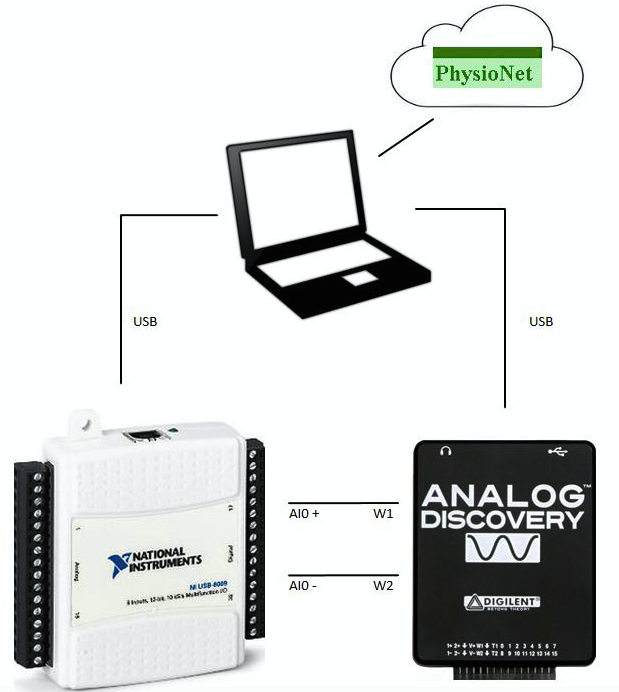
\includegraphics[width=0.8\textwidth]{Figurer/Snip20150427_1}
	\caption{Grafisk illustration af hardware opsætning}
\end{figure}

\subsection{BDD}

\begin{figure}[H]
	\centering
	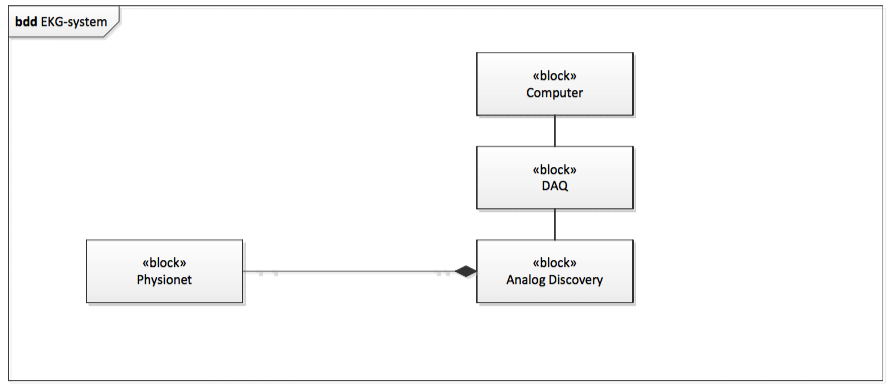
\includegraphics[width=1\textwidth]{Figurer/Snip20150427_2}
	\caption{BDD over EKG-system}
\end{figure}

\subsection{Græseflader}
Grænseflader af forbindelserne imellem de forskellige dele af hardwaren. 

\begin{table}[H] 
	\begin{tabularx}{\textwidth}{l l X}
    \toprule
     \textbf{Forbindelse}   & \textbf{Signaltype} & \textbf{Funktionalitet}    \\ \midrule
     DAQ - Computer         & Digital & DAQ'en konverterer det analoge signal til digitalt og videresender det til 							  computeren. Informationen sendes begge veje. \\ 
     					      \addlinespace[2mm]                                                                                                                                                                            
     Computer - Analog Discovery			& Digital & Computeren simulerer et EKG-signal og sender det til Analog Discovery.\\ 
     				    	  \addlinespace[2mm]   				                                                                                                                                                                           
     Analog Discovery - DAQ			   	& Analog & Analog Discovery	 konverterer signalet fra digitalt til analogt og videresender det til 							      DAQ'en.\\  				      
    \bottomrule                                                                                                                   
    \end{tabularx}
    \caption {Beskrivelse af grænseflader.}
    \label{tab:graenseflader}
\end{table}



\section{Software arkitektur}
Kort indledning

\subsection{GUI}

\subsection{UML klassediagram}

\subsection{Appliktationsmodel}
